\documentclass{beamer}              % only frames
%\documentclass[notes=only]{beamer}   % only notes

%\documentclass[notes]{beamer}       % print frame + notes
%\setbeamertemplate{note page}[plain]
%\setbeameroption{show notes on second screen=right}
\usepackage{etex} % fix errors of many pcks @ http://tex.stackexchange.com/a/38609
\usepackage{pgfpages} % for overlay woth notes @ http://tex.stackexchange.com/q/148722


\usepackage[utf8]{inputenc}
\usepackage{amsmath, amsfonts, epsfig, xspace}
%\usepackage{algorithm,algorithmic}
\usepackage{pstricks,pst-node}
%\usepackage{movie15} % multimedia, movie15
\usepackage[movieson]{optional}
\usepackage[normal,tight,center]{subfigure}
\usepackage{booktabs} % book-quality tables
\usepackage{fancybox}

\usepackage[utf8]{inputenc}
\usepackage{amssymb}

% PRESENTATION LANGUAGE
\usepackage[spanish]{babel}

% DEFINITION OF UPC BLUE
\definecolor{upcblue}{rgb}{0.262745098,0.556862745,0.77254902}
\definecolor{MainBlue}{rgb}{0.2,0.2,0.7}
\definecolor{MainGreen}{RGB}{0, 128, 0}
\definecolor{MainRed}{rgb}{0.73,0.08,0.21}
\definecolor{MyBrickRed}{rgb}{0.549, 0.239, 0.271}    
\definecolor{MyStrongRed}{rgb}{0.60, 0, 0.06}    
\definecolor{MyWebBrown}{rgb}{0.6, 0, 0}
\definecolor{MyWebBlue}{rgb}{0.2, 0.2, 1.0}%{0.07, 0.07, 0.53}

% http://en.wikibooks.org/wiki/LaTeX/Hyperlinks
% http://www.math.uakron.edu/~dpstory/tutorial/pdfmarks/hyper.pdf
\usepackage{hyperref} 
\hypersetup{colorlinks, urlcolor=MainBlue, citecolor=MainBlue, linkcolor=MainBlue} % BrickRed, RoyalBlue

% SUB-FIGURES
\setlength{\subfigcapskip}{-.5em}

% Beamer scheme
\usepackage{beamerthemesplit}
\usetheme{thesis}

% BASIC SCHEMES
%\usecolortheme[named=upcblue]{structure}
%\useinnertheme{rounded}
%\useoutertheme{shadow}

% SOME MINOR COLOR CHANGES
%\setbeamercolor{palette primary}{fg=upcblue,bg=white}
%\setbeamercolor{palette quaternary}{fg=white,bg=upcblue}

%% NEW COMMANDS
\newcommand{\Neurochem}{\textsc{NEUROChem} }
\newcommand{\Comedi}{\textsc{Comedi} }
\newcommand{\UPC}{Universitat Polit\`ecnica de Catalunya}

\newcommand{\vvspace}{\vspace{\baselineskip} \\}
\newcommand{\vvvspace}{$ $ \vspace{\baselineskip} \\}

\newcommand{\smaller}{\tiny}

\newcommand{\mancite}[1]{{\scriptsize{\textbf{\color{MainGreen}{[#1] }}}}}

\renewcommand{\emph}[1]{{\color{MainBlue}{#1}}}
\renewcommand{\textit}[1]{{\it{#1}}}

% BIB
\usepackage{natbib}
\def\newblock{}
\newcommand{\mycite}[1]{{\scriptsize{\textbf{\color{MainGreen}{[\citeauthor{#1}, \citeyear{#1}]}}}}}
\renewcommand{\refname}{References}
\renewcommand{\bibname}{References}

% GRAPHICS OPTIONS
\setkeys{Gin}{width=1.0\textwidth}
\graphicspath{{figures/}{images/}}

% INDENT
%\usepackage[parfill]{parskip}

% THE BASIC PRESENTATION INFORMATION
\title[\textnormal{ \hspace{30em} \insertframenumber/\inserttotalframenumber}]{Biomimetic set up for chemosensor-based machine olfaction}
\author[]{Andrey Ziyatdinov}

%\institute{ 
%  { \small Advisor: Dr. Alexandre Perera} \\ \vspace{0.05\linewidth}  SISBIO - CREB - UPC}
\date{29 June, 2011}

% THE LOGO THAT WILL BE USED IN EACH PAGE
%\logo{
%\includegraphics[width=1.25cm]{logos/creb-upc.jpg} \insertframenumber/\inserttotalframenumber
%}

\begin{document}

% THE TITLE FRAME
\begin{frame}[plain]
  % THE HEADER WITH THE UPC AND CREB LOGOS
  \begin{center}
    \begin{tabular}[\textwidth]{lp{1cm}r}
      
\includegraphics[width=1.5cm]{logos/creb.jpg}
      &
      &
      
\includegraphics[width=1.5cm]{logos/upc.jpg}\\
      \texttt{\tiny Centre de Recerca en Enginyeria Biomèdica}
      &
      &
      \texttt{\tiny Universitat Politècnica de Catalunya}
    \end{tabular}
  \end{center}

  \begin{center}
    %\textsc{\LARGE University of Beer}\\[1.5cm]
    \textsc{PhD Thesis in Biomedical Engineering}\\[0.1cm]
    % Title
    {\Large \emph{Biomimetic set up for \\ chemosensor-based machine olfaction}}\\[1.6cm]
  
  \begin{center}
    % Author and supervisor
    \begin{minipage}{0.14\textwidth}
    \begin{flushleft} %\large
      Aspirant: \\
      Adviser: 
    \end{flushleft}
    \end{minipage}
    \begin{minipage}{0.6\textwidth}
    \begin{flushleft} %\large
      Andrey Ziyatdinov \\
      Alexandre Perera i Lluna
    \end{flushleft}
    \end{minipage}
  \end{center}  

    \vfill

    % Bottom of the page
    {4 December, 2014}
  \end{center}

  % THE REST OF THE TITLE
  %\maketitle
\end{frame}

\begin{frame}
  \frametitle{Outline}
  \tableofcontents
\end{frame}

\section{Introduction}

%----------------------------------
% Example of breath analysis
%----------------------------------
\subsection{Examples of breath analysis}

% frame
\begin{frame}
\frametitle{A story from NYT}

\begin{columns}
\column{0.6\textwidth}

The New York Times\\
\href{http://www.nytimes.com/2006/01/17/health/17dog.html}{Dogs Excel on Smell Test to Find Cancer}\\
By Donald G. McNeil Jr., 2006

\begin{block}{}
Five dogs were trained to detect lung cancer in the breath of patients 
{\scriptsize (N = 138)}
with 99\% accuracy 
\mycite{Mcculloch2006}
%{\scriptsize The Pine Street Clinic, CA}
% (tumors contain alkanes and benzene compounds)
\end{block}

\column{0.3\textwidth}
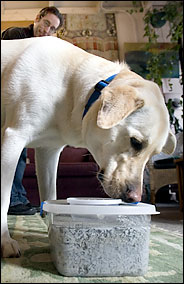
\includegraphics[width=.9\linewidth]{images/dog.jpg} \\
{\tiny Kobi in a cancer-detection experiment}
\end{columns}

Keys to success
\begin{itemize}
  \item Known biomarkers are volatile organic compounds, e.g. alkanes 
  \item Dogs detect odors in the very low parts-per-billion (ppb) range
  \item `Pattern recognition' by means of the canine olfactory system
\end{itemize}  

\end{frame}

% frame
\begin{frame}
\frametitle{An engineering solution}

\begin{columns}
\column{0.6\textwidth}

The colorimetric sensor array consisted of 36
chemically sensitive dots (e.g. metalloporphyrins)
impregnated on a disposable cartridge.

\begin{block}{}
A moderate accuracy of a random forest classifier 
with 73\% sensitivity and 72\% specificity
{\scriptsize (N = 143)}
\mycite{Mazzone2007}
\end{block}

\column{0.3\textwidth}
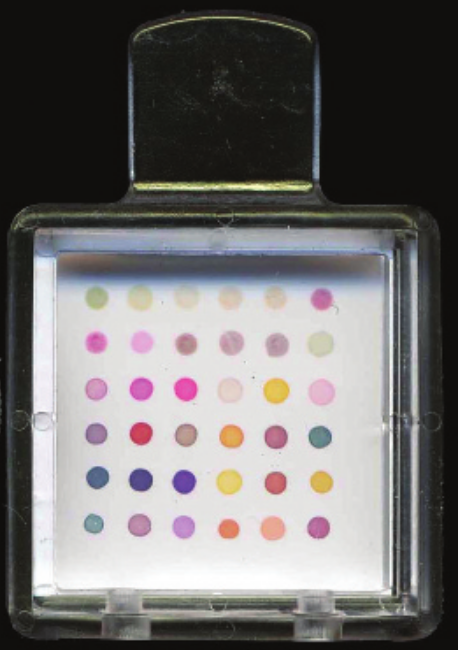
\includegraphics[width=.9\linewidth]{images/colorimetric-sa-2.png} \\
{\tiny 36 chemically sensitive spots}
\end{columns}

System principles
\begin{itemize}
  \item 36 composites were selected to be generally responsive
  \item Such systems perform at up to ppb range for specific volatiles
  \item The identity of the key VOCs has not been clearly established
  \item Hypothesis: an array is able to  detect the unique pattern of VOCs
\end{itemize}  

\end{frame}

\note{
  Colorimetric sensors are composed 
  of different chemically sensitive compounds, e.g. metalloporphyrins.
  Gas absorption causes a change in the color producing a response. 
}

% frame
\begin{frame}
\frametitle{Biomimetic context}

\begin{center}
  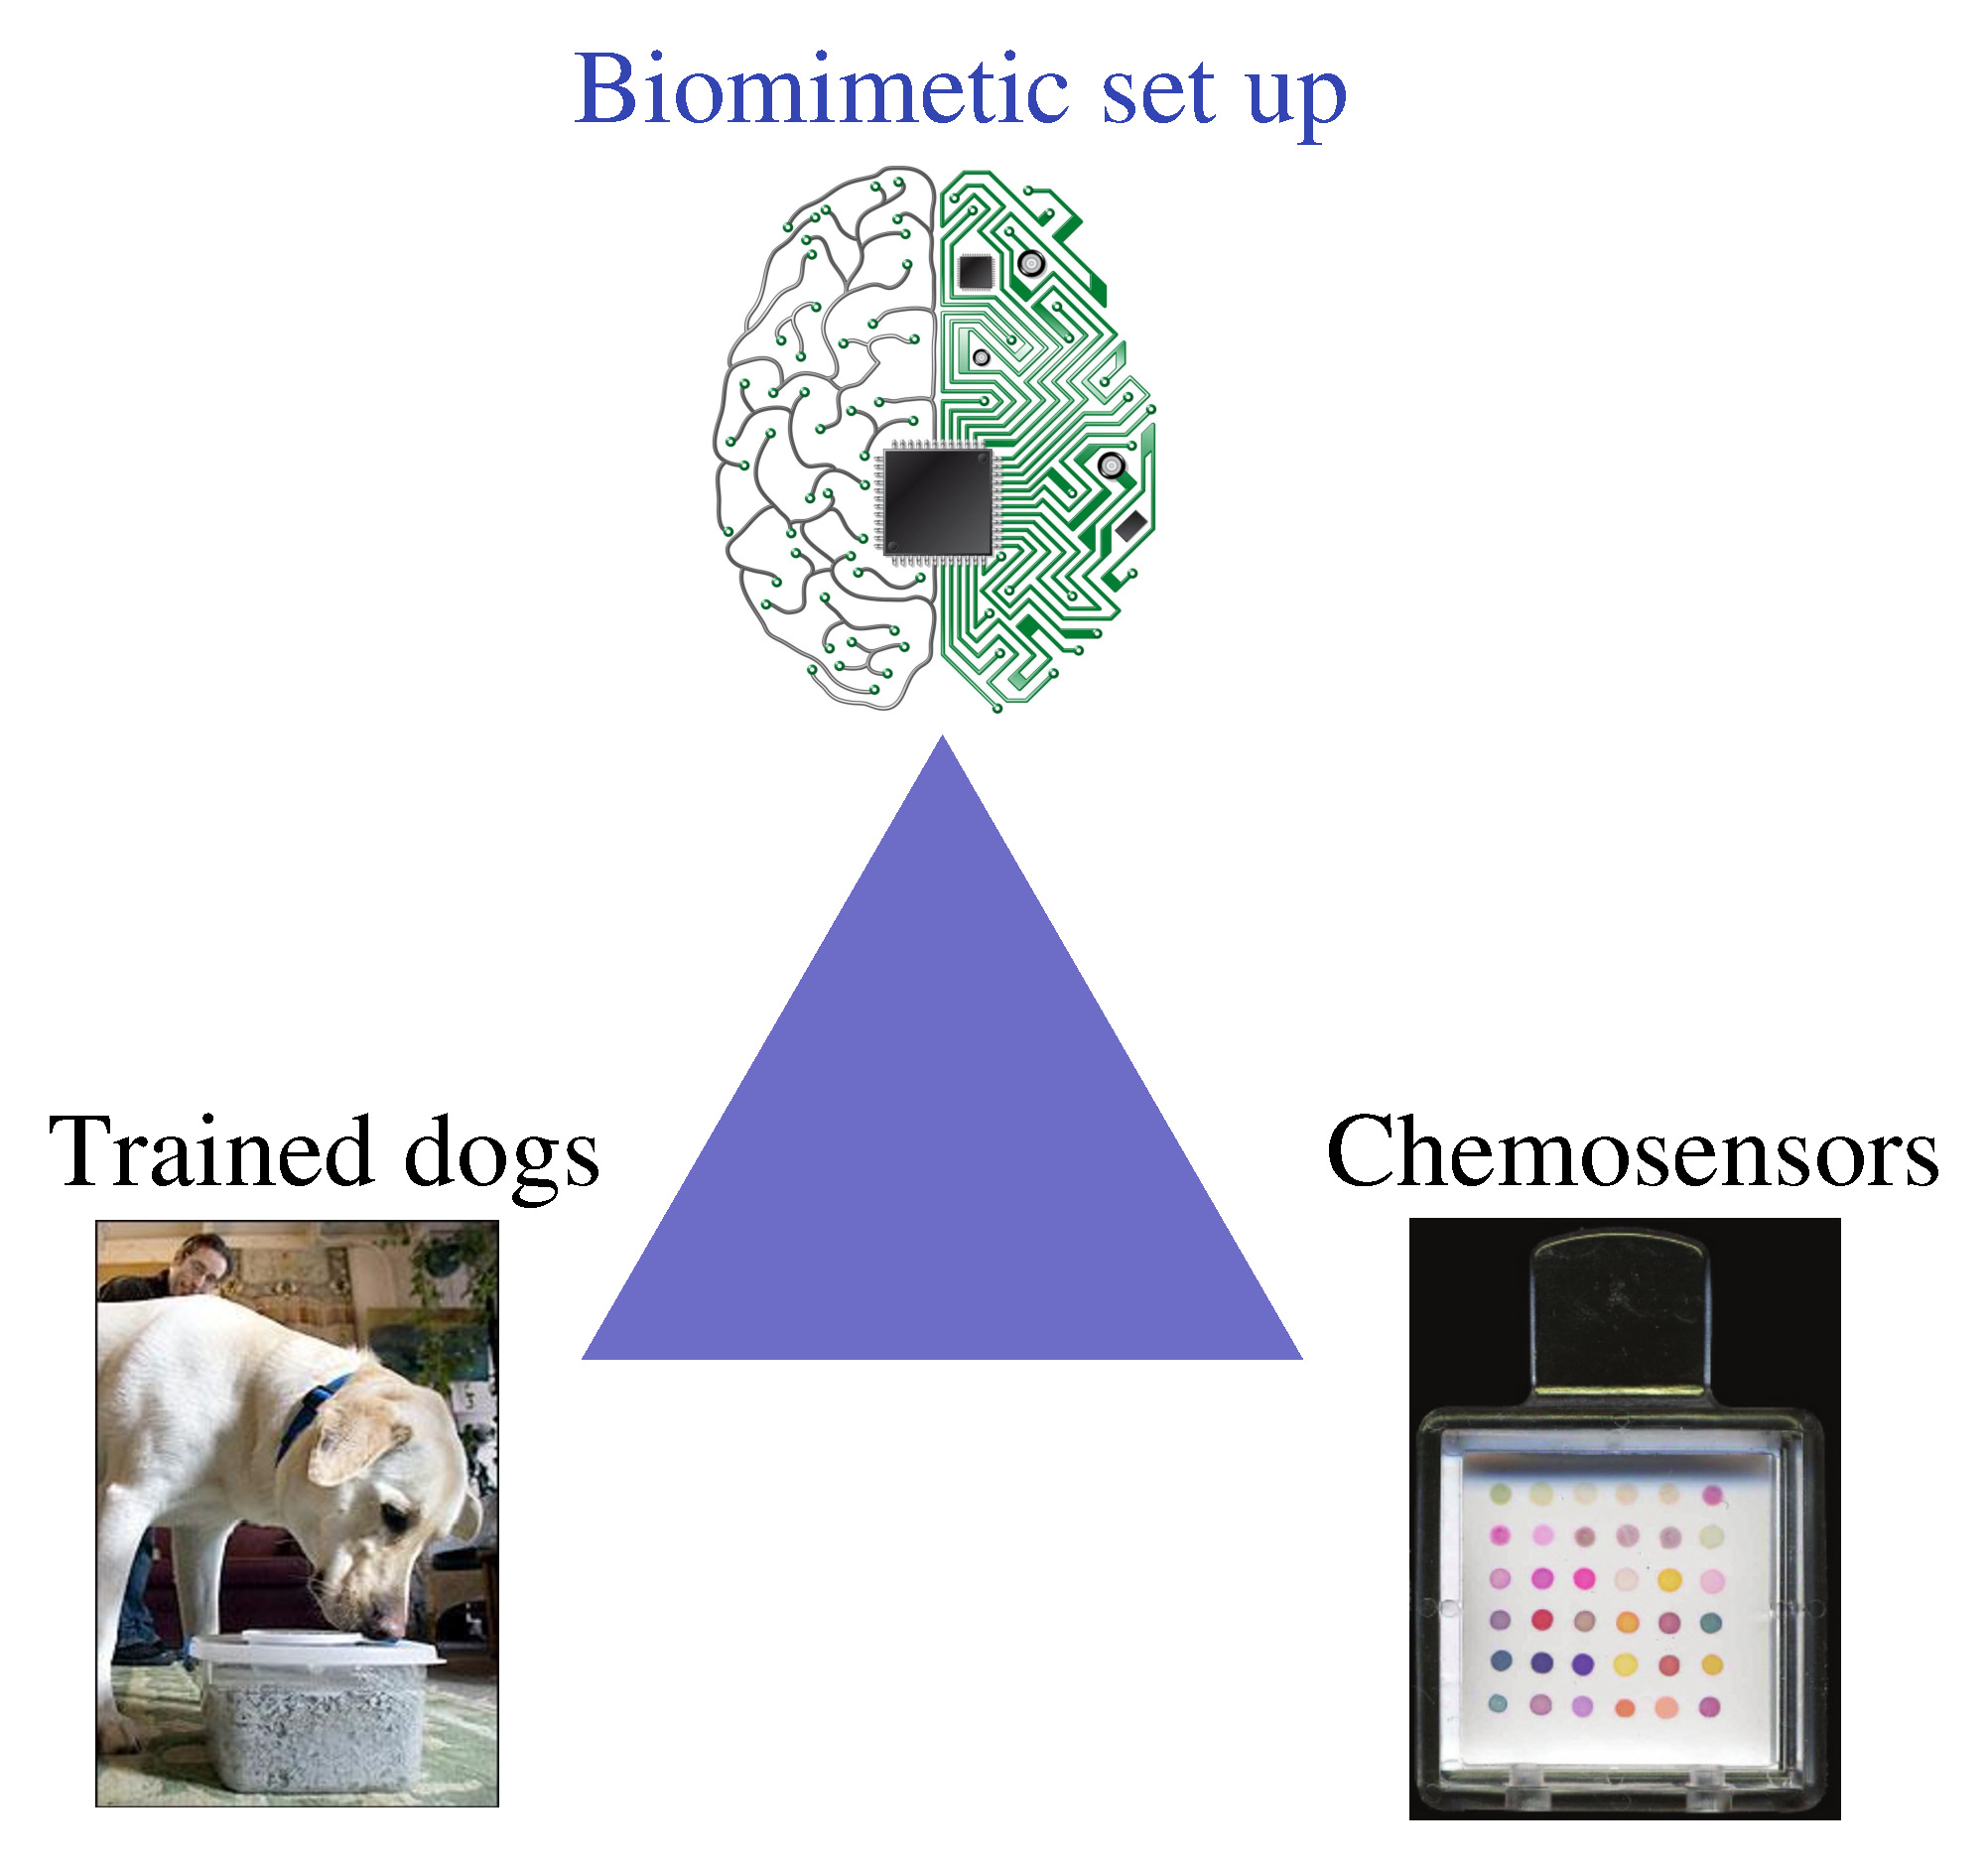
\includegraphics[width=.7\linewidth]{figures/biomimetic-triangle.pdf}
\end{center}
\end{frame}

% frame
\begin{frame}
\frametitle{Biomimetic context}

\begin{center}
  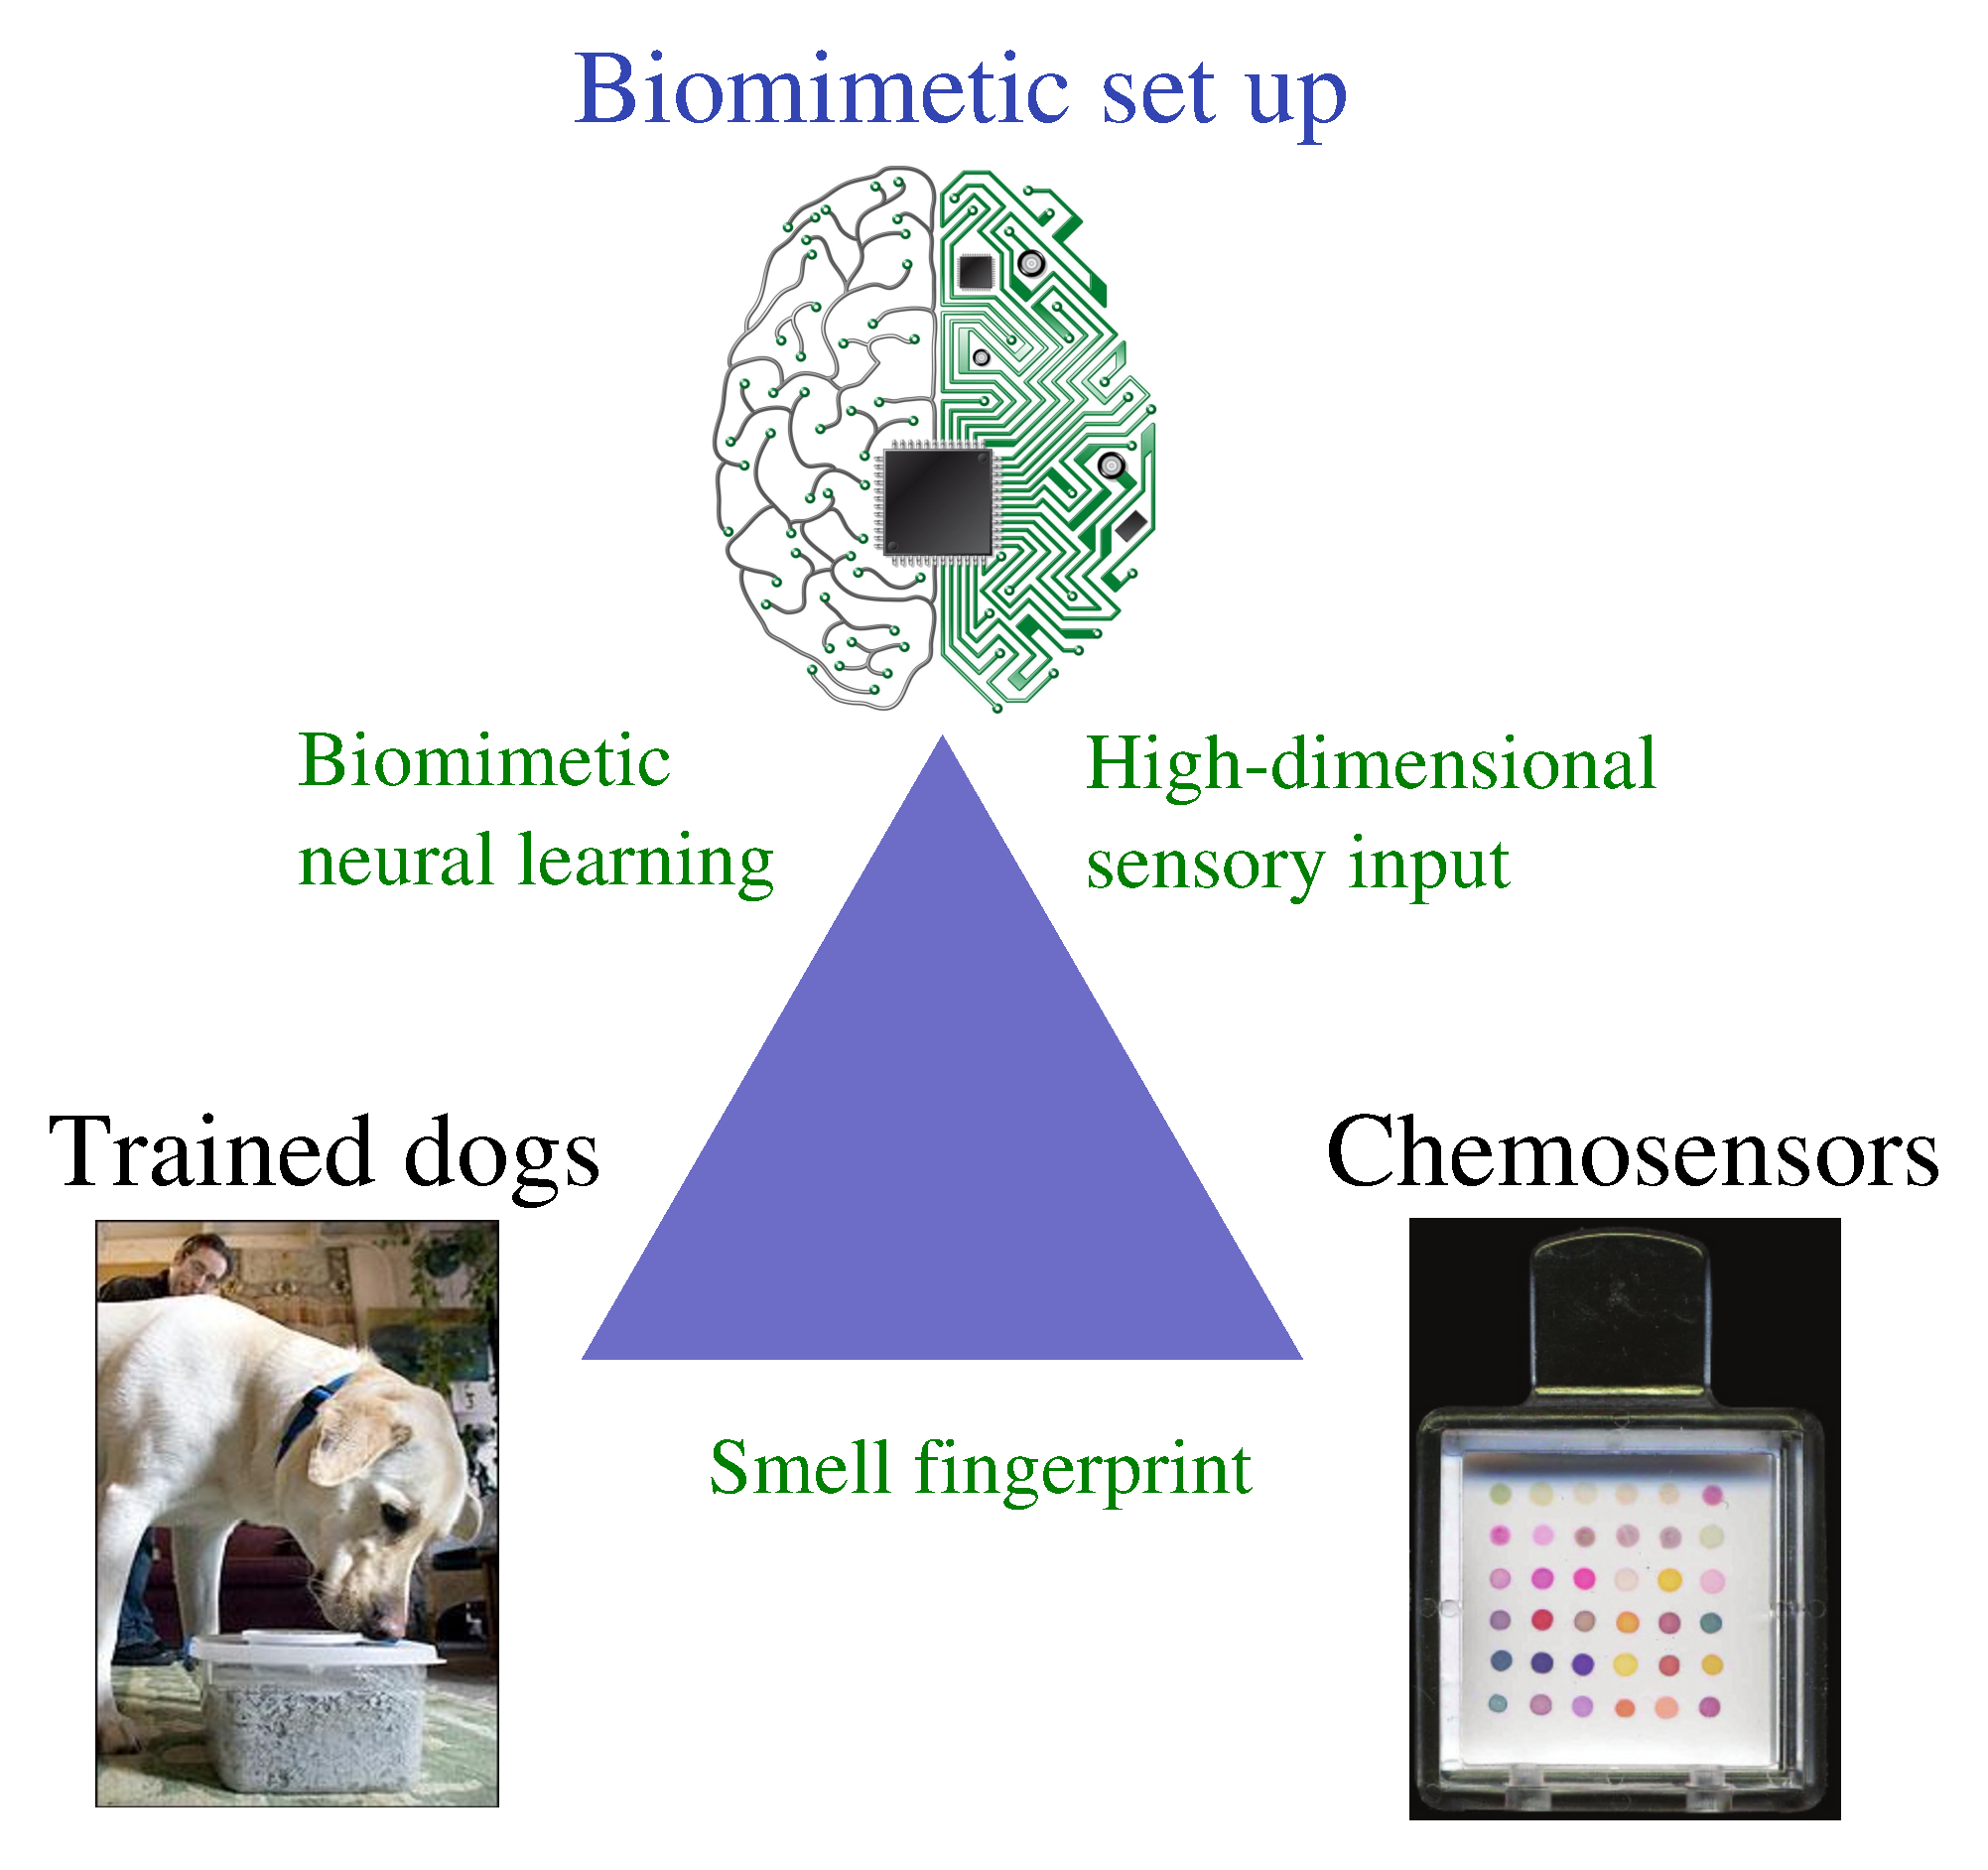
\includegraphics[width=.7\linewidth]{figures/biomimetic-triangle-2.pdf}
\end{center}
\end{frame}

%----------------------------------
% Machine olfaction
%----------------------------------
\subsection{Machine olfaction}

% frame
\begin{frame}
\frametitle{First proposal}

\begin{columns}
\column{0.6\textwidth}
First proposed by Krishna Persaud and George Dodd in 1982 \mycite{Persaud1982}

\begin{block}{}
  ``... we suggest that to make fine
  discriminations between \emph{complex odorant mixtures} containing
  varying ratios of odorants without the necessity for highly
  specialized peripheral receptors, the olfactory systems makes
  use of feature detection using \emph{broadly tuned receptor cells}
  organized in a convergent neuron pathway. 
  ''
\end{block}

\column{0.3\textwidth}
\begin{center}
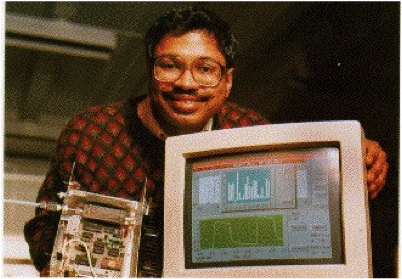
\includegraphics[width=.9\linewidth]{images/krishna.png} \\
{\tiny Prof. K. Persaud and the e-nose}
\end{center}
\end{columns}
\end{frame}


% frame
\begin{frame}
\frametitle{Machine olfaction device}
\begin{description}[leftmargin=0cm]
  \item[By definition:] Arrays of broadly-selective chemical sensors combined with a pattern recognition engine
  \item[Technologically:] A low-cost alternative to instruments of analytical chemistry (or expert panels)
  \item[Conceptually:] Attempt to mimic the biological olfactory system
\end{description}

\begin{center}
  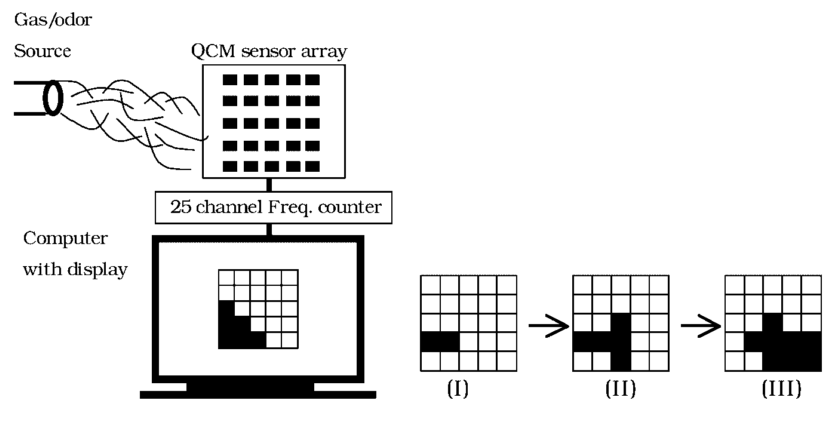
\includegraphics[width=.75\linewidth]{images/array-measurements-handbook.png} \\
  \tiny{\mycite{Pearce2003}}
\end{center}
\end{frame}

% frame
\begin{frame}
\frametitle{Machine olfaction device}
\begin{description}[leftmargin=0cm]
  \item[Gas delivery system] Prepare and deliver samples to sensors
  \item[Array of gas sensors] From chemical-physical quantities to signals
  \item[Interface electronics] Operation and digital-to-analog conversion
  \item[Data processing unit] Digital signals to information pieces
\end{description}

\begin{center}
  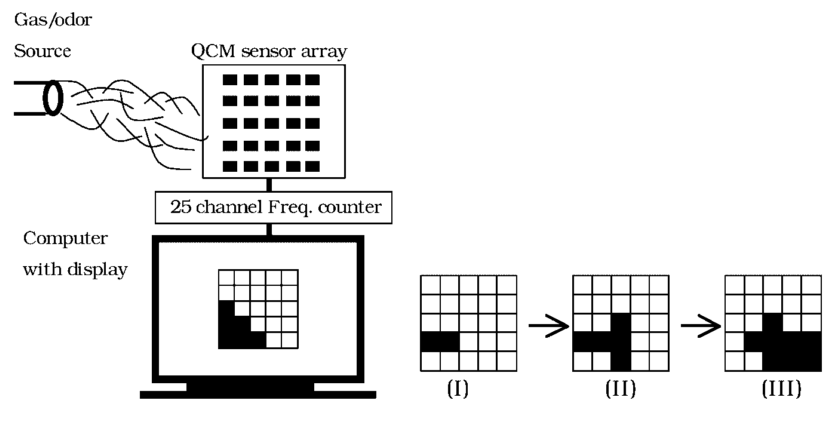
\includegraphics[width=.75\linewidth]{images/array-measurements-handbook.png} \\
  \tiny{\mycite{Pearce2003}}
\end{center}
\end{frame}

%%% Findings in biology
% frame
\begin{frame}
\frametitle{Findings in biology}

\begin{columns}
\column{0.45\textwidth}
\mycite{Persaud1982}

\column{0.45\textwidth}
\mycite{Mori1999}
\end{columns}

\begin{columns}
\column{0.45\textwidth}
\begin{center}
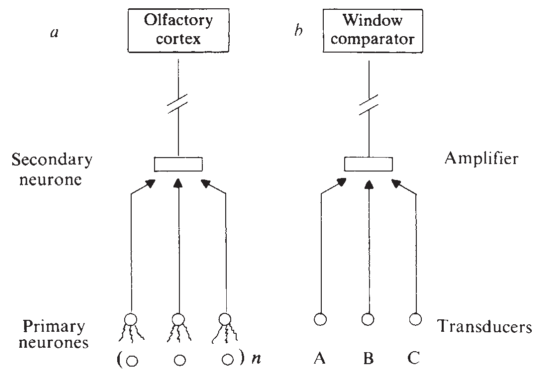
\includegraphics[width=1.1\linewidth]{images/olf-scheme.png} \\
\end{center}

\column{0.45\textwidth}
\begin{center}
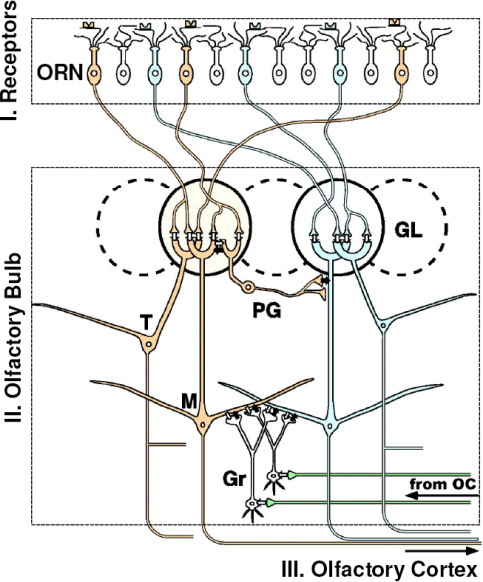
\includegraphics[width=.9\linewidth]{images/olf-pathway-scheme.png} \\
\end{center}
\end{columns}
\end{frame}

% frame
\begin{frame}
\frametitle{Findings in biology}
\begin{columns}

\column{0.45\textwidth}

Early findings
\begin{itemize}
  \item Seven trans-membrane proteins %mediate the chemical-electrical transduction through ORNs
  \mycite{Buck1991} {\scriptsize{\textbf{\color{MainGreen}{(The Nobel Prize)}}}}
  \item Receptors (ORNs) respond to odotopes %odourant molecular features % e.g. carbon-change length, benzene rings, etc
  \mycite{Shepherd1987}, \mycite{Shepherd1994}
  \item Ordered convergence to glomeruli (GL) % ordered projection of ORN into spherical regions (
  \mycite{Vassar1994}
\end{itemize}

\column{0.45\textwidth}
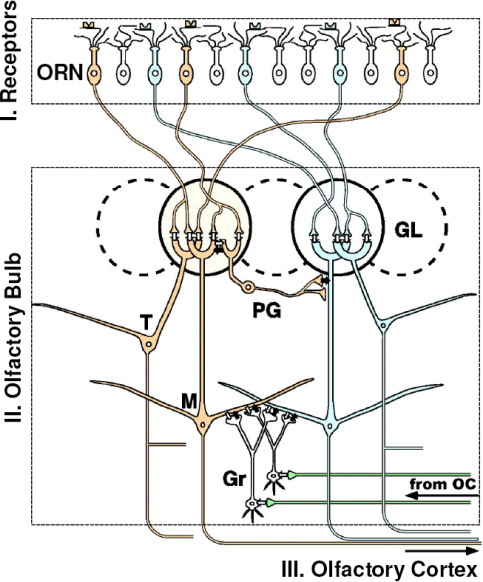
\includegraphics[width=0.9\linewidth]{images/olf-pathway-scheme.png}\\
\mycite{Mori1999}
\end{columns}
\end{frame}

% frame
\begin{frame}
\frametitle{Bioinspired data processing}

First neuromorphic models {\scriptsize (in silico)}
\begin{itemize}
  \item Convergent architecture for increased sensitivity \mycite{Pearce2001}
  \item Dimensionality-reduction technique inspired by ORN convergence \mycite{Perera2006}
  \item Concentration normalization with a model in Olfactory Bulb (OB) \mycite{Raman2006c}
  \item Increasing separability by Hebbian/anti-Hebbian learning rule \mycite{Gutierrez-Galvez2006}

\end{itemize}

\vspace{0.05\linewidth}

First neuromorphic chips
\begin{itemize}
  \item Implementation of the insect macroglomerular complex in Antenal Lobe (AL) \mycite{Pearce2013}
\end{itemize}
\end{frame}

% frame
\begin{frame}
\frametitle{Neuromorphic classifier on iris data set}

\begin{itemize}
  \item Rapidly converged to a representation
  \item The correct association established after a few spikes
  \item Slightly worse performance vs. a naive Bayes classifier
  \item Especially reliable classification in class-overlapped samples
\end{itemize}

\begin{center}
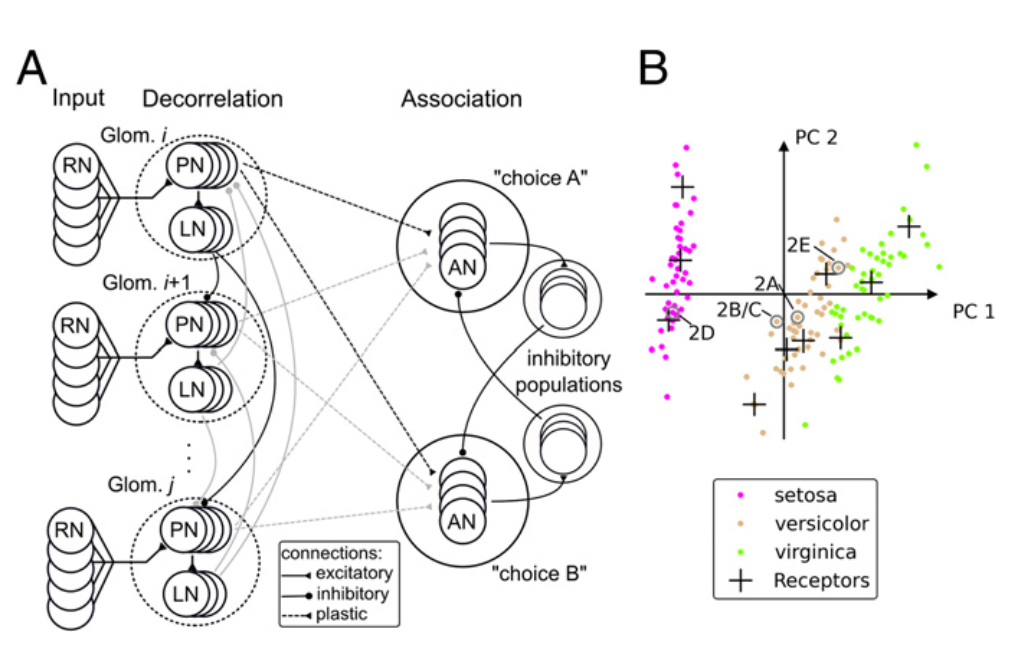
\includegraphics[width=0.65\linewidth]{iris-neuromorphic-chip.png} \\
\mycite{Schmuker2014}
\end{center}

\end{frame}
%----------------------------------
% Thesis background
%----------------------------------
\subsection{Thesis background}

% frame
\begin{frame}
\frametitle{Thesis background}

Topics on the focus of this presentation
{\scriptsize (related to the thesis' contributions)}

\begin{itemize}
  \item Biomimetic robots for machine olfaction
  \item Drift model
  \item Data simulations and benchmarks
\end{itemize}

\vspace{0.05\linewidth}

Topics related to the thesis
\begin{itemize}
  \item Biological olfaction (Section 1.1.2 in the thesis manuscript)
  \item Conducting polymer sensors (Section 1.2.1)
  \item Signal processing (Sections 1.3.1 -- 1.3.3) 
  \item Bioinspired signal processing (Section 1.3.5)
\end{itemize}
\end{frame}

% frame
\begin{frame}
\frametitle{Implementation of biomimetic robots}

\begin{minipage}{0.9\textwidth}
\begin{block}{Target}
  Autonomous robots with embedded computations
  to resolve real-world scenarios like odor source localization
\end{block}
\end{minipage}

\vspace{0.05\linewidth}

Open issues
\begin{itemize}
  \item Low number of gas sensors in arrays
  \item Neuromorphic computations accomplished remotely
  \item Design of neuromorphic chips is still a challenge
\end{itemize}

\vspace{0.05\linewidth}

Existing solutions
\begin{itemize}
  \item Neural simulator IQR (software tool)
  \item Mobile robotic platforms with multimodal sensing
  \item Embedded technology for personal computers (PC)
  \item Unix-like operating systems (OS)
\end{itemize}
\end{frame}

% frame
\begin{frame}
\frametitle{Drift phenomenon}

\begin{minipage}{0.9\textwidth}
\begin{block}{General definition}
  Gradual changes in a quantitative characteristic 
  that is assumed to be constant over time
\end{block}
\end{minipage}

%  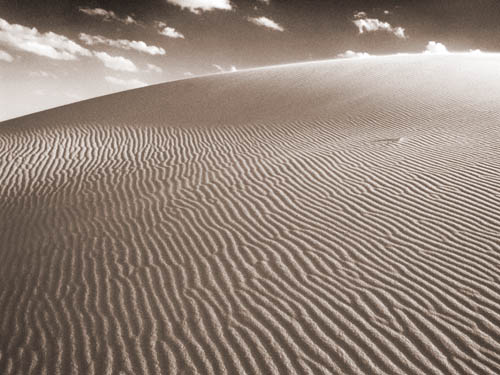
\includegraphics[width=0.9\textwidth]{wind-sand-sky.jpg}
  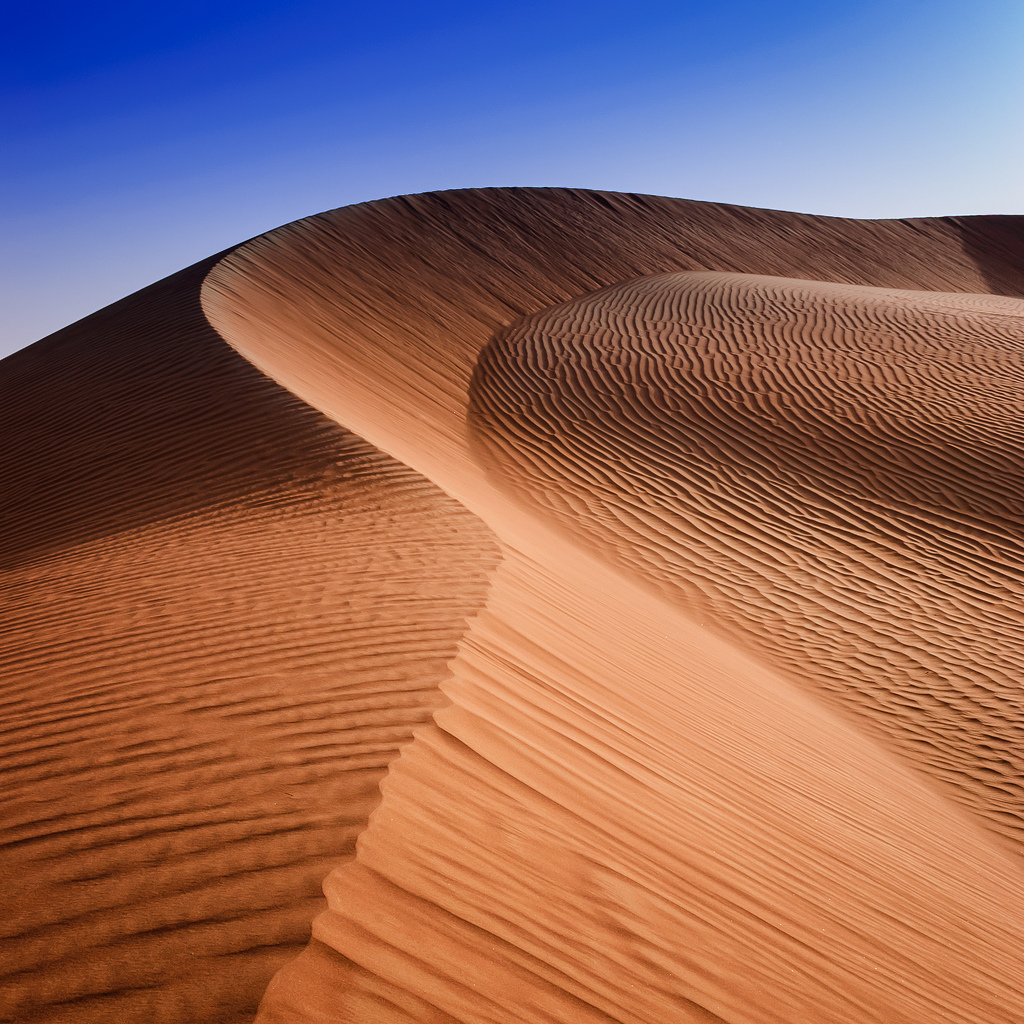
\includegraphics[width=0.9\textwidth]{images/sand.jpg} \\
  \mancite{Figure source: https://www.flickr.com/photos/michaelkeith/6905715219/}
\end{frame}

% frame
\begin{frame}
\frametitle{Drift in chemosensors}

\begin{minipage}{\textwidth}
\begin{block}{Instrumentation long-term noise (similar to batch effects)}
  Complex and inevitable effect due to several sources:
  sampling protocol, environmental conditions, etc.
\end{block}
\end{minipage}

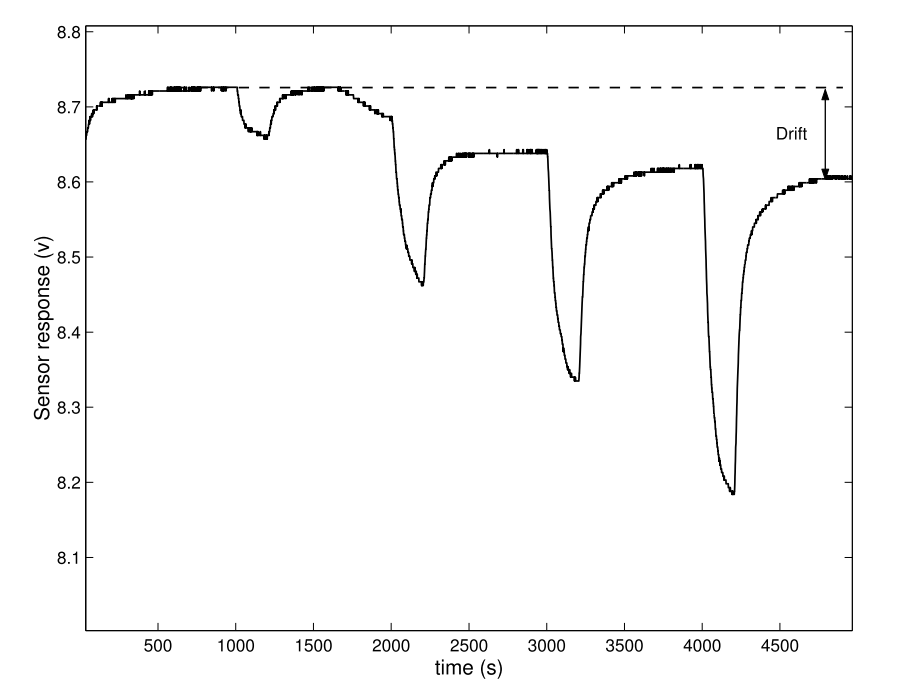
\includegraphics[width=0.6\textwidth]{images/add-drift.png} \\
\mycite{Bermak2005}

\end{frame}

% frame
\begin{frame}
\frametitle{Multivariate correction of drift}

A reference method of Component Correction (CC) \mycite{Artursson2000}

\begin{itemize}
  \item Drift is a subspace $\mathbf{V}$ of variance common to all classes
  \item $\mathbf{V}$ is estimated by PCA performed on samples from a reference gas
  \item The drift noise is removed by CC:
  \begin{equation*}
    \mathbf{X'} = \mathbf{X} - (\mathbf{X}\mathbf{V})\mathbf{V}^T
  \end{equation*}
\end{itemize}

\begin{columns}
  \column{0.45\textwidth}
  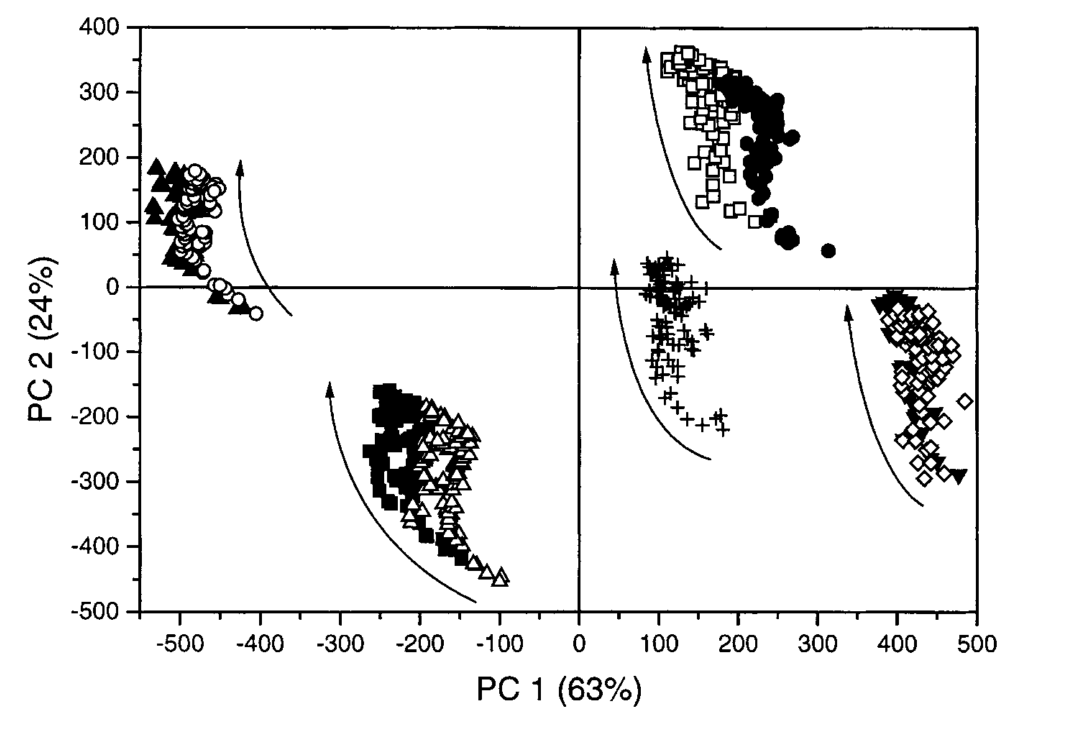
\includegraphics[width=\textwidth]{images/mvar-drift-1.png}
  \column{0.45\textwidth}
  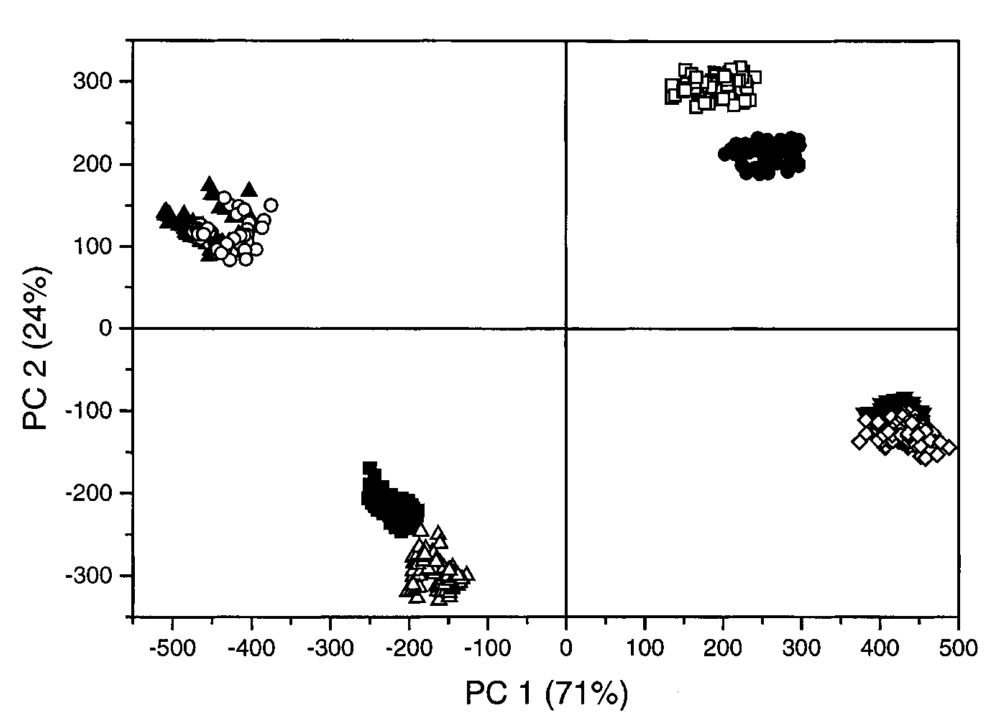
\includegraphics[width=\textwidth]{images/mvar-drift-2.png}
\end{columns}
\mycite{Artursson2000}
\end{frame}

% frame
\begin{frame}
\frametitle{Data availability}

Benchmarks
\begin{itemize}
  \item First time mentioned Ricardo Gutierrez-Osuna in a review \mycite{Gutierrez-Osuna2002}
\end{itemize}

\vspace{0.05\linewidth}

Public data sets
\begin{itemize}
  \item The need for public data was discussed in the ISOEN 2011
  \item Lab of Ramon Huerta (UCSD, USA) was the first in publishing data sets
  at The UCI Machine Learning Repository 
  \href{https://archive.ics.uci.edu/ml}{https://archive.ics.uci.edu/ml}
  (4 data sets to date)
\end{itemize}

\vspace{0.05\linewidth}

Data simulations
\begin{itemize}
  \item Many sensor models were published, but there is no any data simulation 
  tool available to the comunity
\end{itemize}


\end{frame}

%----------------------------------
% Objectives and Methods
%----------------------------------
\section{Goals and Methods}

% frame
\begin{frame}
\frametitle{Thesis goals}

\end{frame}

% frame
\begin{frame}
\frametitle{Robot implementation}

\end{frame}

% frame
\begin{frame}
\frametitle{UNIMAN data set}

\end{frame}

%----------------------------------
% References
%----------------------------------

\begin{frame}[allowframebreaks]
  \frametitle{Bibliography}
  \nocite{*}
  \bibliographystyle{apalike} % plainnat
  {\scriptsize 
    \bibliography{thesis}
  }
\end{frame}

\end{document}



